\subsection{Erfassung und Verarbeitung von Messwerten}
\subsubsection{Kapazitive Feuchtigkeitsmessung}

Zur Feuchtigkeitsmessung des Substrats wird ein kapazitiver Sensor verwendet. Die genaue Herleitung der Funktionsweise würde den Umfang dieser Arbeit übersteigen.

\smallskip

Der genutzte Sensor \citep{Sensor} gibt die gemessene Feuchtigkeit als eine Spannung zwischen 0V und 3V aus und wird mit einer Spannung von 3.3V betrieben - dem 
selben Spannungspegel mit welchem auch die \ac{uC} betrieben werden. Dies vereinfacht die Verwendung immens.

\smallskip

Verbunden wird der Sensor mit dem Anschluss PA1 des STM32, welcher wiederum prozessorseitig mit dem \ac{ADC} verbunden ist \citep{STM32_Datasheet} und auf der Platine mit 
Pin 15 verknüpft ist \citep{IoTGateway}. Desweiteren sind Verbindungen zur Versorgungsspannung und dem Massepotential erforderlich \citep{Sensor}.



\subsubsection{Analog-Digital Converter}

Es wird ein einzelner Kanal des ADC1 des STM32s verwendet. Dieser wird so konfiguriert, dass eine einzelne Konversion durch Software ausgeführt wird und bei Abschluss
dieser ein Interrupt ausgelöst wird \citep{STM32_Ref}. Die Konfiguration geschieht mittels CubeMX \citep{CubeMX}.

\begin{figure}[h]
    \centering
    \begin{subfigure}{0.45\textwidth}
        \centering
        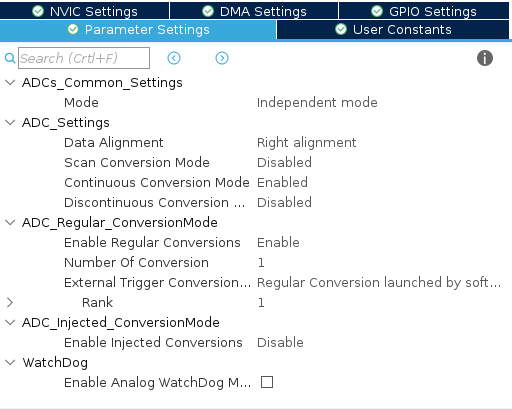
\includegraphics[width=\textwidth]{Pictures/adc_param.png}
        \caption{Parameter ADC}
        \label{img: Parameter ADC}
    \end{subfigure}
    %
    \begin{subfigure}{0.45\textwidth}
        \centering
        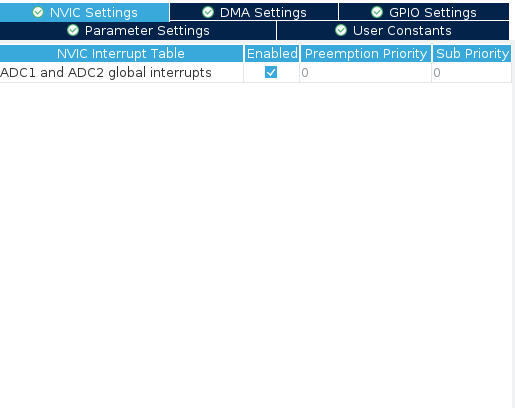
\includegraphics[width=\textwidth]{Pictures/adc_nvic.png}
        \caption{ADC Interrupt}
        \label{img: ADC Interrupt}
    \end{subfigure}
    \caption{Konfiguration des \acp{ADC}}
    \label{img: ADC config}
  \end{figure}

  Der \ac{ADC} verfügt über die Funktion der Selbstkalibration \citep{STM32_Ref}. Diese wird während der Initialisierung des \ac{uC} mittels folgender Funktion durchgeführt \citep{HAL_Description}:
  \begin{lstlisting}[caption={\textit{ADC Kalibrierung}}]
    HAL_ADCEx_Calibration_Start(&hadcx);      
  \end{lstlisting}

  \newpage

  Die Verarbeitung des  Interrupts des \ac{ADC} wird ähnlich realisiert, wie in \ref{subsub: Empfang} für den \ac{UART} in beschrieben. Nach dem Auftreten eines 
  Interrupts wird dieser in der Routine
  \begin{lstlisting}
    void HAL_ADC_ConvCpltCallback(ADC_HandleTypeDef *hadc)
  \end{lstlisting}  
  verarbeitet. 

  \smallskip

  Die Konversion wird mittels der Funktion \lstinline!HAL_ADC_Start_IT(&hadcx)! gestartet und kann mittels \lstinline!HAL_ADC_Stop_IT(&hadcx)! gestoppt werden.

  \subsubsection{Strukturvariable SENS\_STRUCT}
  Auch hier wird aus Gründen der Übersichtlichkeit eine Strukturvariable mit diversen Flags und Variablen eingeführt.
  \begin{lstlisting}[caption={\textit{Sensor Strukturvariable}}]
    typedef struct
    {
        uint8_t cal_flag;						
        uint16_t dry_value;			
        uint16_t wet_value;			
        volatile uint8_t timer_flag;	
        uint16_t an_value;			
        uint8_t percentage;			
        volatile uint8_t adc_flag;	
        uint8_t send_flag;			 
    } SENS_STRUCT;
  \end{lstlisting}

  Das Flag \lstinline!cal_flag! zeigt an, dass der Sensor kalibriert wurde. Das Flag \lstinline!adc_flag! wird genutzt, um eine vollendete Konversion des \ac{ADC} anzuzeigen.
  Um die kontinuierliche Übertragung von Messwerten freizuschalten wird \lstinline!send_flag! genutzt. \lstinline!timer_flag! speichert, ob ein Interrupt durch einen
  Timer ausgelöst wurde.

  \smallskip
  Die Variablen \lstinline!dry_value!, \lstinline!wet_value! und \lstinline!an_value! speichern Werte zur Kalibrierung sowie den aktuellen Messwert. Dessen Repräsentation
  in Prozent wird mittels der Variable \lstinline!percentage! gespeichert.

  \subsubsection{Kalibrierung des Sensors}

  Der Sensor muss vor Benutzung Kalibriert werden, damit eine zuverlässige Messung möglich ist. Dazu muss ein Messwert erfasst werden, wenn der Sensor komplett trocken
  ist und ein Messwert, wenn der Sensor in Wasser getränkt ist \citep{Sensor}. 

  \smallskip

  Die Kalibrierung wird durch den Befehl CALIBRATE, beschrieben in \ref{subsub: Nachricht}, ausgelöst. Da der Sensor für die Messung der Werte in Wasser getaucht werden muss,
  muss der Nutzer durch den Prozess begleitet werden. Dies geschieht durch die Benutzung der auf der Platine aufgelöteten LED \citep{IoTGateway}, welche abhängig vom aktuellen
  Schritt aufleuchtet. 
  Die Funktion \lstinline!uint8_t cal_sens(ADC_HandleTypeDef hadc, SENS_STRUCT * sens)! in der Datei \lstinline!sensor.c!
  implementiert die Kalibrierung. Die Funtkion gibt eine '1' bei Erfolg oder eine '0' bei Misserfolg zurück.
  
  \smallskip

  Der Ablauf lautet wie folgt:
  \begin{itemize}
      \item Starten der Kalibrierung durch CALIBRATE
      \item LED an, Sensor muss trocken sein
      \item LED aus, Wert wird gemessen
      \item LED an, Sensor muss nass sein
      \item LED aus, Wert wird gemessen 
  \end{itemize}

  Um zuverlässige Messwerte zu erhalten, werden immer 10 Messungen durchgeführt und die gemessenen Werte gemittelt. Die Messung wird exemplarisch für den Messwert des
  trockenen Sensors erklärt. Der Zähler \lstinline!cal_counter! speichert die Anzahl der Messungen. Die Variable \lstinline!dry! speichert den gemittelten Messwert.
  \begin{lstlisting}[caption={\textit{Kalibrationsroutine}}]
    HAL_ADC_Start_IT(&hadc);
    while(cal_counter<10)								
    {
	    if(sens->adc_flag == 1)
        {
            cal_counter ++;
            sens->an_value = hadc.Instance->DR;
            dry += sens->an_value;
            sens->adc_flag=0;
            HAL_ADC_Start_IT(&hadc);
        }
    }
    cal_counter = 0;
    dry = dry / 10;			
    sens->dry_value = dry;
  \end{lstlisting}

  Die Messung wird durch \lstinline!HAL_ADC_Start_IT(&hadc)! gestartet. Wenn die Konversion abeschlossen ist, wird in der entsprechenden Interruptroutine das Flag 
  \lstinline!adc_flag! gesetzt. Anschließend wird der Zähler, welcher die While-Schleife der Messung steuert, inkrementiert und der aktuelle Messwert aus dem Register
  des \ac{ADC} ausgelesen. Dieser Messwert und seine folgenden Messwerte werden in der Variable \lstinline!dry! summiert. 

  \smallskip

  Nach dem Rücksetzen des Flags wird eine erneute Konversion gestartet, bis der Zähler seinen Endwert erreicht hat. Anschließend wird der Zähler rückgesetzt, der Messwert
  gemittelt und an die Strukturvariable weitergegeben.

  \smallskip

  Die LED für die Benutzerinformation wird mittels eines Timers (siehe \ref{subsub: Timer}), genauer TIM2, mit einer Periodendauer von 0.5s gesteuert. Der Timer wird mit 
  \lstinline!HAL_TIM_Base_Start_IT(&htimx)! gestartet \citep{HAL_Description}. In seiner Interruptroutine wird das Flag \lstinline!timer_flag! gesetzt. 
  \begin{lstlisting}[caption={\textit{LED Timer}}]
    HAL_TIM_Base_Start_IT(&htim2);								 
    while(sens->timer_flag)
    {
        HAL_GPIO_WritePin(LED_GPIO_Port, LED_Pin, GPIO_PIN_SET);
    }
    sens->timer_flag = 0; 												
    HAL_GPIO_WritePin(LED_GPIO_Port, LED_Pin, GPIO_PIN_RESET);
  \end{lstlisting} 
  Mittels der While-Schleife, wird gewartet, bis der Timer seinen Interrupt ausgelöst hat und das entsprechende Flag gesetzt wurde. Innerhalb der Schleife, wird
  die LED angeschalten. Sobald die Schleife verlassen wurde, also der Interrupt ausgelöst und somit das Flag gesetzt wurde, wird das Flag rückgesetzt und die LED
  wieder abgeschalten.

  \smallskip

  Innerhalb der Interruptroutine wird der Timer wieder gestoppt, um ein ständiges Auslösen des Interrupts zu vermeiden.

  

  \subsubsection{Berechnung des Messwertes}
  Mittels der durch die Kalibrierung ermittelten Werte lässt sich nun der eigentliche Messwert auf eine Skala von 0\% bis
  100\% darstellen. Die Variable \(x\) steht für den aktuellen Messwert, während \(x_{wet}\) und \(x_{dry}\) für die jeweiligen Kalibrationswerte stehen. 

  \smallskip 

  Die Formel, welche den Zusammenhang darstellt ergibt sich zu:
  \smallskip

  \begin{math}
        f(x)=100-\frac{(x-x_{wet})*100}{x_{wet}-x_{dry}}
  \end{math}

  Bei der Implementation dieser Funktion in C ist bei der Nutzung von Integervariablen ohne Vorzeichen darauf zu achten, dass der Nenner nicht negativ oder null wird,
  da dies zu unerwarteten Ergebnissen führen kann.

  \smallskip

  Die Funktion \lstinline!uint8_t val_sens(ADC_HandleTypeDef hadc, SENS_STRUCT * sens)! implementiert die Berechnung und ist in Datei \lstinline!sensor.c! zu finden.
  Um die bereits erwähnten Ergebnisse zu vermeiden, wird geprüft, ob die Differenz zwischen den Kalibrierungswerten nicht negativ ist. Als Rückgabewert wird die 
  gemessene Feuchtigkeit in Prozent ausgegeben.

  \begin{lstlisting}[caption={\textit{Berechnung des Messwerts}}]
    uint8_t val_sens(ADC_HandleTypeDef hadc, SENS_STRUCT * sens)
    {
        uint8_t percentage;
        sens->an_value = HAL_ADC_GetValue(&hadc);
        if(sens->an_value-sens->wet_value > 0)										
        {
            percentage = 100-((sens->wet_value-sens->an_value)*100)
            /(sens->wet_value-sens->dry_value);
        }
        else
        {
            percentage = 0;
        }
        return percentage;
    }
  \end{lstlisting}
